\chapter{Teoria Elementar dos Conjuntos}
Durante os capítulos vamos falar de conjuntos e seus elementos, que são os objetos de estudo da teoria dos conjuntos. Essa área da matemática é uma forma consistente e frequentemente utilizada para fundamentar todas as outras, servindo como um tipo de linguagem interna.
\margem{Em comparação com outras áreas da matemática, a Teoria dos Conjuntos é recém nascida. A Geometria, por exemplo, é estudada desde a Idade Antiga.}

A teoria dos conjuntos é uma área recente da matemática, seu desenvolvimento data do final do século XIX, sendo seu estágio inicial muito controverso, marcado pelas críticas do matemático alemão Kronecker e os paradoxos encontrados pelo filósofo e matemático Betrand Russell.
\section{Conceito}
Um conjunto é um agrupamento, uma coleção de objetos. Todos os objetos dessa coleção são chamados de \emph{elementos} e a relação entre o conjunto e o elemento é a \emph{pertinência}, isso é, quando dizemos que um elemento pertence a um conjunto, queremos dizer que o elemento é um objeto daquela coleção.

Entretanto, isso não é uma definição, mas apenas uma noção vaga. Ao invés de definirmos o que são conjuntos, elementos ou o que significa pertinência, vamos descrever propriedades que nos dizem como esses três conceitos se comportam, exatamente como fazemos com o conceito de ponto, reta e plano em geometria.

\definicao{ 
São \textbf{conceitos primitivos}:
\label{PrimitivosConjuntos}
\begin{enumerate}[1)]
\item Conjunto
\item Elemento
\item Pertinência 
\end{enumerate}
}


\exem{Alguns conjuntos}{
\begin{enumerate}[a)]
\item Conjunto dos estados brasileiros do sudeste
\item Conjunto das cores do arco-íris
\item Conjunto dos números pares
\item Conjunto das vogais
\item Os números (naturais) menores que $50$
\end{enumerate}
Os elementos que pertencem a esses conjuntos são (respectivamente) 
\begin{enumerate}[a)]
\item São Paulo, Rio de Janeiro, Espírito Santo e Minas Gerais
\item Vermelho, Laranja, Amarelo, Verde, Azul, Anil e Violeta
\item 0, 2, 4, 6, 8, 10, 12, 14, \ldots
\item a, e, i, o , u
\item 0,1,2,\ldots,48,49
\end{enumerate}
}
O conjunto das vogais é formado pelos elementos a, e, i, o, u. Para simbolizar o fato de que $a$ é um elemento do conjunto \emph{Vogais} (que $a$ pertence a \emph{Vogais}) nós escrevemos\\ $$a \in \text{\emph{Vogais} (lê-se "a pertence a \emph{Vogais}")}$$\\Da mesma forma, podemos escrever\\ $$b \notin \text{\emph{Vogais} (lê-se "b não pertence a \emph{Vogais}")}$$\\para dizer que $b$ não pertence ao conjunto das vogais.

\margem{Repare que os elementos podem ser eles mesmos conjuntos! Por exemplo, o conjunto dos estados do sudeste é composto por estados, que são conjuntos de cidades.}
\subsection{O conjunto vazio}
O conjunto mais simples possível de se formar é aquele sem elementos, que chamamos de conjunto vazio. Para representarmos esse agrupamento utilizamos um símbolo especial, o $\emptyset$. O conjunto vazio pode ser pensado como uma caixa vazia: ele existe, mas não há nada dentro dele. Assim como o conceito de conjunto, elemento e pertinência, nós aceitamos a existência do conjunto vazio.

\definicao{ \textbf{Conjunto Vazio} \\ 
\begin{center}
O Conjunto Vazio ($\emptyset$) é o único conjunto que não possuí elementos
\end{center}
}
\section{Denotando Conjuntos}
\subsection{Enumeração}


Exitem algumas formas de se denotar conjuntos. Quando o conjunto tem poucos elementos é fácil e prático apenas listar seus elementos. Descrevemos o conjunto dessa forma escrevendo seus elementos entre chaves ($\{$ e $\}$).
\exem{Descrevendo conjuntos por enumeração}{
$$\text{\emph{Vogais}} = \{a,e,i,o,u\}$$Da mesma forma poderíamos escrever $$\text{\emph{Cores}} = \{\text{Vermelho, Laranja, Amarelo, Verde, Azul, Anil, Violeta}\}$$}Sempre utilizando o sinal de igualdade e as \emph{chaves} ($\{$ e $\}$). Quando usamos essa notação não faz diferença quantas vezes aparece um elemento. Por exemplo, o conjunto $$A = \{a,b,c,d\}$$é o mesmo que o conjunto$$A =\{a,b,b,b,a,c,d,c,d,\}$$Isso quer dizer que \textbf{essa notação não serve para designar quantidade ou ordenação dentro de um conjunto}.

O conjunto vazio agora pode ser escrito de outra forma

$$\emptyset = \{\}$$

\margem{Enumerar os elementos só é adequado quando o conjunto é pequeno, mas frequentemente comete-se um \textit{abuso de linguagem} e escreve-se conjuntos grandes (ou mesmo infinitos) como um tipo de enumeração, usando alguma regra de formação implícita.}

Também podemos descrever os conjuntos segundo alguma regra que fique subentendida.

\exem{Abusos de linguagem na enumeração}{Se chamarmos o conjunto dos números pares de P, poderíamos escrever $$P = \{2,4,6,8,\ldots\}$$

Se chamarmos de $<_{50}$ o conjunto dos números menores que 50, poderíamos escrever $$<_{50} = \{0,1,\ldots,48,49\}$$}

Essa forma, entretanto, necessita que o leitor do texto advinhe qual é a regra de formação do conjunto. Como pessoas diferentes podem advinhar coisas diferentes, não é estritamente correta.
\subsection{Especificação}
Para representar de forma não ambigua um conjunto infinito ou muito grande, podemos descrevê-lo através de uma \textbf{propriedade} e um \textbf{conjunto maior que o contenha}. Assim, poderíamos representar o conjunto dos números pares da seguinte forma\margem{O conjunto $\mathbb{N}$ (que será visto nos próximos capítulos) é o conjunto dos números naturais, que possui todos os números inteiros positivos}$$P = \{ n \in \mathbb{N} | \text{ o resto da divisão de } n \text{ por } 2 \text{ é } 0\}$$ (lê-se "n pertence aos naturais e o resto da divisão de n por 2 é 0")

Nesse caso, o conjunto maior que continha $P$ era $\mathbb{N}$(os números naturais) e a propriedade que designava o conjunto era '$\text{ o resto da divisão de } n \text{ por } 2 \text{ é } 0$'. 

O conjunto dos números menores que $50$ escrito da mesma forma que o conjunto anterior é:$$<_{50} = \{ n \in \mathbb{N} | n < 50\}$$(lê-se "n pertence aos naturais e n é menor que 50")
O conjunto que contém $<_{50}$ é o mesmo que contém $P$, os números naturais, mas dessa vez a propriedade é diferente. A propriedade que caracteriza os elementos de $<_{50}$ é que seus elementos são todos menores que $50$.

Vamos ver um exemplo de como usar essa notação em outras situações. \margem{Descrever um conjunto apenas pela propriedade de seus elementos, sem especificar um conjunto maior que o contenha, foi o motivo de vários paradoxos aparecerem na teoria dos conjuntos. Se pudessemos fazer isso, considere o seguinte conjunto: $$U=\{x | x \notin x\}$$Uma análise rápida nos diz: $U \in U$ somente se $U \notin U$, voilà nosso paradoxo!}
\exem{Especificando conjuntos através de uma propriedade}{
Seja $P$ o conjunto de todas as pessoas. Se quiséssemos representar o conjunto de todos os homens poderíamos escrever: $$H = \{h \in P \ | \ h\text{ é homem}\}$$Se quiséssemos além disso especificar o conjunto dos homens que praticam tênis, poderíamos escrever: $$T = \{h \in H \ | \ h \text{ pratica tênis}\}$$Ou então, igualmente poderíamos escrever:$$T = \{h \in P \ | \ h \text{ é homem e pratica tênis}\}$$} É importante salientar que sempre é necessário especificar um conjunto maior que contenha o conjunto que desejamos descrever, para usarmos essa notação.
\section{Inclusão e Igualdade}
\subsection{Inclusão}
Acabamos de criar a noção de conjunto e nós gostaríamos que ela fosse útil para expressarmos algumas relações entre objetos que desejamos organizar. Um fato recorrente em organizações é de que, às vezes, um conjunto está \textit{dentro} do outro. Por exemplo, em Biologia, na organização científica dos seres-vivos, todo ser-vivo que é um \emph{mamífero} é necessariamente um \emph{animal}. Na matemática isso ocorre com muita freqüência. Por exemplo, todo número par (2,4,6,8, etc) é um número inteiro. Descrevemos esse fato dizendo que \emph{Mamíferos} é subconjunto de \emph{Animais} e escrevemos $$\text{\emph{Mamíferos}} \subset \text{\emph{Animais} (lê-se "Mamíferos está contido em Animais")}$$ou então$$\text{\emph{Animais}} \supset \text{\emph{Mamíferos} (lê-se "Animais contém Mamíferos")} $$Por outro lado, também é verdade que nem todos os \emph{Animais} são \emph{Mamíferos}. Escrevemos $$\text{\emph{Animais}} \not \subset \text{\emph{Mamíferos} (lê-se "Animais não está contido em Mamíferos")}$$Agora que a idéia de inclusão está clara, precisamos expressar essa noção intuitiva dentro da linguagem que criamos, isto é, precisamos expressar o que acabamos de criar em função dos \textit{conceitos primitivos} (\ref{PrimitivosConjuntos}). Isso pode ser conseguido da seguinte forma:

\definicao{\textbf{Subconjunto}\\
Dizemos que $A \subset B$ se todo elemento de $A$ é um elemento de $B$

Ou em linguagem simbólica $$ (A \subset B) \Leftrightarrow (\forall x (x \in A \Rightarrow x \in B))$$}
\marginpar{
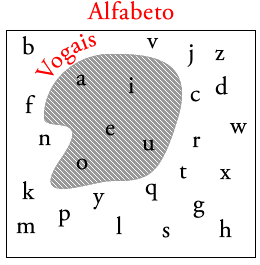
\includegraphics[width=0.85\marginparwidth]{imagens/alfabetoconjunto.png}
	\captionof{figure}{O conjunto \emph{Vogais} é subconjunto do conjunto \emph{Alfabeto}}
	\label{fig:subconjuntovogais}}
	
Vamos conferir algumas propriedades da inclusão para $A$, $B$ e $C$ quaisquer: 

\caixaprop{
\begin{propriedade}[Reflexiva] $A \subset A$ 
\end{propriedade}
\begin{propriedade}[Transitiva] Se $A \subset B$ e $B \subset C$ então $A \subset C$ 
\end{propriedade}
\begin{propriedade}
$\emptyset \subset A$
\end{propriedade}
}

\exem{Inclusão de Conjuntos}{Se $A =\{1,2,3,4,5\}$, $B = \{1,2,6,7,8\}$, $C=\{6,7,8\}$, $D = \{1,2,3\}$, então:
\begin{enumerate}[1)]
\item $C \subset B$
\item $D \subset A$
\item $C \not\subset A$ (Isso quer dizer: "C não é subconjunto de A")
\item $D \not\subset B$
\end{enumerate}
}
\subsection{Igualdade}
Com a idéia de \emph{subconjunto}, podemos definir o que significa dizer que um conjunto é igual a outro. Por exemplo, o conjunto dos números que não são ímpares é exatamente o conjunto dos números pares. A idéia por trás desse conceito é que todo número que não é ímpar é par e também, todo número que é par, não é ímpar. Ou seja, o que nós estamos fazendo na verdade é mostrando que um conjunto é subconjunto do outro. Assim:

\definicao{\textbf{Igualdade}

Dizer $A = B$ é o mesmo que dizer $A \subset B$ e $B \subset A$

Ou, em linguagem simbólica$$(A=B)\Leftrightarrow ((A \subset B) \land (B \subset A))$$}

\margem{Essa caracterização da igualdade entre conjuntos leva a uma propriedade que devemos destacar, a extensionalidade. A propriedade da \emph{extensionalidade} diz que um conjunto é caracterizado por seus elementos. Isso é, se dois conjuntos têm exatamente os mesmos elementos, então eles são iguais.}
\section{Operações entre Conjuntos}
Quando temos dois agrupamentos, podemos fazer certas mudanças nos mesmos de forma a respeitar algumas propriedades. Podemos, por exemplo, criar um único grupo formado pelos outros dois, ou selecionar apenas os elementos que fazem parte dos dois conjuntos. Por exemplo, imagine o conjunto dos países que falam espanhol e o conjunto dos países da América do Sul. É uma pergunta natural "Quais países da américa do sul falam espanhol?". Para esse tipo de situação, podemos fazer operações entre os conjuntos, criando um terceiro conjunto a partir de dois pré-existentes. Vamos falar um pouco sobre algumas operações possíveis.
\subsection{União}
Dados dois conjuntos, podemos estar interessados em saber qual é conjunto formado pelos elementos dos dois conjuntos. O conjunto dos números naturais, por exemplo, é a união do conjunto dos números ímpares com os números pares. De forma geral, quando temos dois conjuntos $A$ e $B$ denotamos o conjunto cujos elementos são todos os de $A$ e de $B$ por $A \cup B$ (lê-se "A união B"). 

\definicao{\textbf{União}

Dados dois conjuntos $A$ e $B$ existe o conjunto $A\cup B$ e
$$x \in (A \cup B) \text{ se e somente se } x\in A \text{ e/ou } x \in B$$
}
\marginpar{
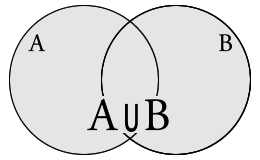
\includegraphics[width=0.85\marginparwidth]{imagens/aub.png}
	\captionof{figure}{Representação no diagrama de Venn-Euler de $A\cup B$}
	\label{fig:aubvenneuler}}
\caixaprop{
Para quaisquer conjuntos $A$ e $B$, temos:
\begin{propriedade}
$A \cup A = A$
\end{propriedade}
\begin{propriedade}
$A \cup B = B \cup A$
\end{propriedade}
\begin{propriedade}
$A \cup \emptyset = A$
\end{propriedade}
\begin{propriedade}
$A \subset A \cup B$
\end{propriedade}
\begin{propriedade}
$A \cup (B \cup C) = (A \cup B) \cup C$
\end{propriedade}}
\subsection{Intersecção}
\marginpar{
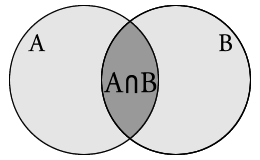
\includegraphics[width=0.85\marginparwidth]{imagens/aeb.png}
	\captionof{figure}{Representação no diagrama de Venn-Euler de $A\cap B$}
	\label{fig:aebvenneuler}}
	\marginpar{
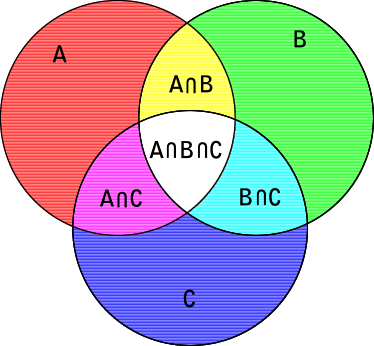
\includegraphics[width=0.85\marginparwidth]{imagens/aebec.png}
	\captionof{figure}{Intersecção de três conjuntos no diagrama de Venn-Euler}
	\label{fig:aebec}}
A intersecção é a operação que representa o ato de escolher os elementos que estão simultaneamente nos dois conjuntos. O problema sugerido dos países no início da seção é um caso típico de problema de intersecção. De forma geral, quando temos dois conjuntos $A$ e $B$ denotamos o conjunto cujos elementos são os de $A$ e de $B$ simultaneamente por $A \cap B$ (lê-se "A intersecção B"). 
\definicao{\textbf{Intersecção}

Dados dois conjuntos $A$ e $B$ existe o conjunto $A\cap B$ e
$$x \in (A \cap B) \text{ se e somente se } x\in A \text{ e } x \in B$$}


Algumas propriedades. Para quaisquer conjuntos $A$ e $B$, temos:
\margem{Dizemos que dois conjuntos são \textit{disjuntos} se a sua intersecção for vazia, isso é, $A\cap B = \emptyset$.}
\caixaprop{
\begin{propriedade}
$A \cap A = A$
\end{propriedade}
\begin{propriedade}
$A \cap B = B \cap A$
\end{propriedade}
\begin{propriedade}
$A \cap \emptyset = \emptyset$
\end{propriedade}
\begin{propriedade}
$A \cap B \subset A$
\end{propriedade}
\begin{propriedade}
$A \cap (B \cap C) = (A \cap B) \cap C$
\end{propriedade}
\begin{propriedade}
$A \cap (B \cup C) = (A \cap B) \cup (A \cap C)$
\end{propriedade}
\begin{propriedade}
$A \cup (B \cap C) = (A \cup B) \cap (A \cup C)$
\end{propriedade}
}

\subsection{Diferença ou Complementar}
Na seção sobre inclusão,\marginpar{
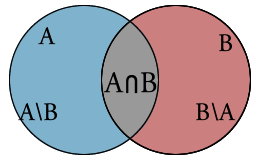
\includegraphics[width=0.85\marginparwidth]{imagens/amenosb.png}
	\captionof{figure}{Em azul o conjunto $A\setminus B$ e em vermelho o conjunto $B\setminus A$, representados no diagrama de Venn-Euler}
	\label{fig:amenosb}} nós vimos que \emph{Animais} $\not \subset$ \emph{Mamíferos}. Poderíamos estar interessados em descrever o conjunto dos \emph{Animais} que não são \emph{Mamíferos}. Com o que vimos até agora (União e Intersecção) isso não é possível. Para suprir essa necessidade, criamos o conceito de \emph{diferença} entre conjuntos. O que queremos é que o conjunto diferença entre $A$ e $B$ tenha exatamente aqueles elementos de $A$ que não pertencem a $B$.

Geralmente denotamos a diferença entre $A$ e $B$ por $A \setminus B$. Com menos frequência aparece também a notação $A - B$. Continuando com a nossa política de reduzir tudo aos conceitos primitivos, definimos:
\margem{Repare que na maioria das vezes não é verdade que $A \setminus B = B \setminus A$.}

\marginpar{
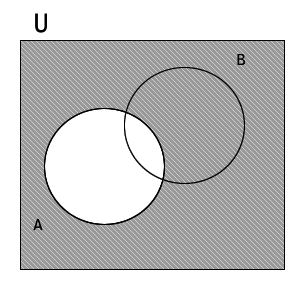
\includegraphics[width=0.85\marginparwidth]{imagens/acomp.png}
	\captionof{figure}{Em cinza o conjunto $A^c$}
	\label{fig:acompb}}
	\marginpar{
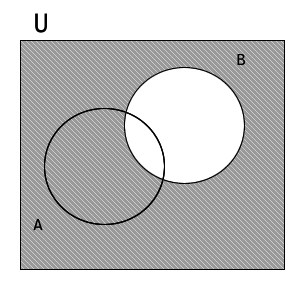
\includegraphics[width=0.85\marginparwidth]{imagens/bcomp.png}
	\captionof{figure}{Em cinza $B^c$}
	\label{fig:bcompa}}
\marginpar{
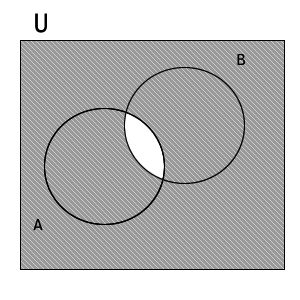
\includegraphics[width=0.85\marginparwidth]{imagens/ainterb.png}
	\captionof{figure}{Em cinza $(A\cap B)^c$, que é também $A^c \cup B^c$}
	\label{fig:ainterb}}
\marginpar{
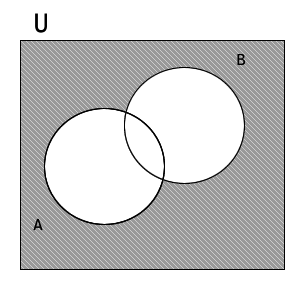
\includegraphics[width=0.85\marginparwidth]{imagens/auniaobcomp.png}
	\captionof{figure}{Em cinza $(A\cup B)^c$, que é também $A^c \cap B^c$}
	\label{fig:auniaobcomp}}
\definicao{\textbf{Diferença entre Conjuntos}
$A \setminus B$ é o conjunto dos elementos que pertencem a $A$ e não pertencem a $B$
ou, de forma equivalente
$$A \setminus B = \{x \in A \ | \ x \notin B\}$$
}


 Algumas propriedades da diferença entre dois conjuntos:
\caixaprop{
\begin{propriedade}
$A \setminus A = \emptyset$
\end{propriedade}
\begin{propriedade}
$A \setminus \emptyset = A$
\end{propriedade}
\begin{propriedade}
$A \setminus B = A \setminus (A \cap B)$
\end{propriedade}
\begin{propriedade}
$(A \setminus B) \subset A$
\end{propriedade}
\begin{propriedade}
$(A \setminus B) \cap B = \emptyset$
\end{propriedade}
}

Existe um caso particular de diferença entre conjuntos que será mais interessante para nós na maioria das vezes, que é quando estamos trabalhando sobre um conjunto universo, que é um conjunto maior do que todos os outros sob os quais estamos operando. Se $U$ for o conjunto universo e $A$ for um subconjunto de $U$ ($A \subset U$), podemos escrever $A^c$ para representar $U \setminus A$.Também é utilizado $\overline{A}$ com o mesmo significado. Cuidado: A notação do complementar só faz sentido quando está claro qual é o conjunto universo.
Algumas propriedades do complemento:
\caixaprop{
\begin{propriedade}
$A^c \cap A = \emptyset$
\end{propriedade}
\begin{propriedade}
$\emptyset^c = U$
\end{propriedade}
\begin{propriedade}
$U^c = \emptyset$
\end{propriedade}
\begin{propriedade}
$A^c \cap B^c = (A\cup B)^c$
\end{propriedade}
\begin{propriedade}
$A^c \cup B^c = (A\cap B)^c$
\end{propriedade}
}